%TC:group tabular 1 1
%TC:group table 1 1

\chapter{Preparation}

\paragraph{} This chapter shall first address the refinements made to the project proposal. Then I shall explain the tests that were performed to establish Excel's suitability for musical development. Next, the design decisions for Excello shall be explained. The software engineering tools and techniques employed will then be introduced. Finally, the research that was conducted to decide to implement a converter from MIDI to Excello shall be summarised.

\section{Proposal Refinements}

\paragraph{} The project designed a notation by which music can be defined within a spreadsheet along with a system for interpreting the notation in the spreadsheet to produce audio output. This continued to explore ways in which time can be abstracted away from the grid.

\paragraph{} The aim was to implement an Excel add-in subject to successful initial testing. An add-in is a web application displayed within Excel that can read and write to the spreadsheet using the Office Javascript API \footnote{https://docs.microsoft.com/en-us/javascript/api/excel?view=office-js}. Arbitrary additional data and markup can be included in the spreadsheet. Only information in the spreadsheet is required for playback with the add-in. Tests shall be carried out to verify that suitable audio output can be produced for music end-user music programming within Excel to be possible.

\paragraph{} A sizeable addition to the project beyond the initial proposal was to perform participatory design \cite{muller:pd} to advise on improvements that can be made beyond the initial prototype. Participants would be able to identify aspects of the current design that (don't) work well or add cognitive difficulty. The prototype was introduced to users and from this, new features and improvements implemented. A subset of these participants who gain sufficient familiarity with the project were used for more informed summative evaluation. As a result, the proposed extension of incorporating live-coding would only be implemented if deemed high priority by the participants.

\paragraph{} MIDI was the file type for which a converter was implemented to translate to a CSV file for use in Excel. Additional explanation on the choice of MIDI is provided below. It was also motivated by participants who wished to be able to integrate Excello with their use of digital audio workstations such as Logic Pro, Ableton Live, and GarageBand.

\section{Feasibility Analysis}

\paragraph{} The following section outlines the libraries I explored and the tests carried out to assess the feasibility of synthesising notes given data in a spreadsheet using an Excel add-in. All tests were carried out in Excel Online\footnote{https://office.live.com/start/Excel.aspx} using Script Lab\footnote{https://www.microsoft.com/en-us/garage/profiles/script-lab/}, an add-in that allows users to create and test simple add-ins experimenting with the Office Javascript API. These add-ins have an HTML front end and can access libraries and data elsewhere online.

\paragraph{} If add-ins were run in an older version of Internet Explorer, playing sound or using of the Web Audio API would be possible.An add-in that played a wav file verified that an add-in could create sound. \cite{mozilla:webaudioapi}.

\subsection{Note Synthesis Library}

\paragraph{} The Web Audio API allows audio to be synthesised from the browser using Javascript \cite{mozilla:webaudioapi}. Creating a program for users to define and play musical structures requires synthesising arbitrary length, pitch and volume notes. To avoid the lower-level audio components (e.g. oscillators), I researched libraries that would allow me to deal with higher level musical abstractions of the synthesised notes. Sarkar's SheetMusic used the library tones\footnote{https://github.com/bit101/tones}, a simple API where only the pitch and volume envelope\footnote{How the note's volume changes over its duration} of all notes. Other limitations included no definition of volume and only including simple waveform synthesisers.

\paragraph{} Tone.js\footnote{https://tonejs.github.io/} is a library built on top of the Web Audio API providing greater functionality than tones. An \texttt{Instrument} such as a \texttt{Synth} or \texttt{Sampler} is defined. The \texttt{triggerattackrelease} release method of these instruments allows a note of a given pitch, volume and duration to be triggered at a particular time. Notes are defined using scientific pitch notation (SPN) (e.g. \texttt{F\#4}), name (\texttt{F\#}) combined with octave (\texttt{4}). As Script Lab can reference libraries from the Node Package Manager (NPM), I tested playing notes with pitch defined in the add-in Javascript.

\subsection{Office Javascript API}

\paragraph{} For users to produce music within Excel, the musical output must be informed by the data in the spreadsheet. Previous tests created notes defined in the add-in Javascript. To test the Excel API, I played a note with the Tone.js library, the pitch of which was defined in the spreadsheet. This was extended so note playing, not just the pitch, was defined within a cell, detected and executed.

\paragraph{} Next, I was able to play a sequence of constant length notes defined in consecutive cells. The range of cells was accessed using the Excel API and the values were played using the \texttt{Tone.Sequence} object. Having performed these tests, I confirmed Tone.js combined with the Excel API had the functionality required to assist in the implementation of the project.

\section{Excello Design and Language}

\subsection{Abstracting Time}

\paragraph{} Dave Griffith's Al-Jazari \cite{mclean:visualisation} takes place in a three-dimensional world where robotic agents navigate around a two-dimensional grid. The height and colour of the blocks over which the agents traverse determines the sound that they produce. The characteristics of the blocks are modified manually by users at run-time whilst the agents are moving. Whilst there are more complex conditional instructions, the basic instructions have the agents rotate and move forwards and backwards in the direction that they are facing. There exists a dual formalism in both the agent's instructions and the block state. This design is intended to make live coding more accessible, both when viewing performances and becoming a live coder.

\begin{figure}[ht]
  \centerline{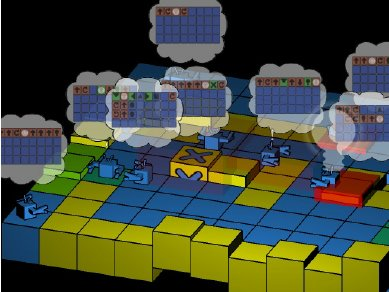
\includegraphics[width=100mm]{figs/alJazari.jpg}}
\caption{Programmed agents moving around a grid in Al-Jazari \textcopyright\ Alex Mclean}
\label{prep:alJazari}
\end{figure}

\paragraph{} In Al-Jazari, the agents are programmed by placing symbols corresponding to different movements in thought bubbles that appear above them. This is not suitable for programming within spreadsheets where all data must exist alphanumerically within cells. If an agent was to continue moving forwards many times in a row, it would become tiresome to keep adding the move forward symbol. This is less of an issue in Al-Jazari where the grid within which the agents navigate only measures ten cells wide and long.

\paragraph{} The concept of having a cursor navigate around a cartesian plane is the method used by turtle graphics. Just as this concept is used in Al-Jazari to play the cell the agents occupy rather than colour it, it is suitable for spreadsheets. The turtle abstraction is employed by Excello by having notes defined in cells and defining agents, known as turtles, to move through the spreadsheet activating them. In order to play a chord, multiple turtles must be defined to pass through multiple cells corresponding to the note of the chord. This method maintains high notational consistency but sacrifices the abstractions for musical structures that are available in languages like Sonic Pi - \texttt{chord(\upquote{F\#}, \upquote{maj7})}. By implementing methods in the add-in to add the notes of chords to the grid, the use of the abstractions is maintained whilst preserving consistency and cleanness in the spreadsheet itself.

\paragraph{} The turtle is the crux of the Logo programming language \cite{goldman:turtle}. In Logo, turtles are programmed entirely by text. for example, \texttt{repeat 4 [forward 50 right 90]} has a turtle move forwards 50 units and turn 90 degrees to the right. This is repeated four times to draw a square. A similar method is employed in Excello but the language is designed to be less verbose.

\subsection{Initial Prototype Design}

\paragraph{} In Excello, notes are placed in the cells of the spreadsheet and pathways through the grid are defined using a language for programming turtle movement. The notes in the cells will be played when a turtle moves through that cell. When the program is run, the melodic lines produced by all turtles defined in the grid will be played concurrently. Turtles are defined with a start cell, movement instructions, the speed with which they move through the grid (cells per minute) and the number of times they repeat their path. As in Al-Jazari, distance in space maps to time \cite{mclean:texture}, Excello extends upon this by allowing different turtles to navigate at different speeds. This allows parts with longer notes to be defined more concisely and for phase music\footnote{Music where identical parts are played at different speeds} to be easily defined.

\paragraph{} As in Logo, turtles begin facing north. The move command \texttt{m} moves the turtle forward one cell in the direction that it is facing. Just like in Logo, the turtle always moves in the direction it is facing. The commands \texttt{l} and \texttt{r} turn the turtle 90 degrees to the left and right respectively. Repeats are implemented in Logo with the command \texttt{repeat} followed by the number of repeats and the instructions to be repeated \cite{goldman:turtle}. In order to create more concise instructions, single commands can be repeated in succession by placing a number immediately after it. For example, the command \texttt{m4} will have the turtle move forwards four cells in the direction that it is facing. The direction a turtle is facing can be defined absolutely using the commands \texttt{n}, \texttt{e}, \texttt{s} and \texttt{w} to face the turtle north, east, south and west. This could have instead moved the turtle in that direction, but this would have lost the consistency that the turtle always moves in the direction it is facing. To change notes' volume, dynamics (\texttt{ppp}, \texttt{pp}, \texttt{p}, \texttt{mp}, \texttt{mf}, \texttt{f}, \texttt{ff}, \texttt{fff}) can be placed within the turtle instructions. Any notes played after this will be played at that dynamic. In the same way the dynamics in western notation are a property of the staff and not individual notes, dynamics were originally designed to be a property of the turtle. In order to repeat multiple instruction sequences, these are placed in brackets and the number of repeats put immediately after the bracket. For example, \texttt{(r m50)4} would define a path going clockwise around a fifty by fifty square. This 8 character example is equivalent to the Logo example above that requires 30 characters. The ability to repeat larger series of instruction is why the relative movements \texttt{l} and \texttt{r} are included in the language despite being less explicit than the compass based directions.

\paragraph{} It may not be convenient for each melodic line to be defined by a single path of adjacent cells. Just as conventional score notation often spans across multiple lines, the splitting of parts is a useful form of secondary notation. This requires the turtle to navigate to non-adjacent cells and then proceed playing. For graphic drawing in Logo, the pen can be lifted, allowing the turtle to navigate without colouring the space beneath it. This is suitable for a graphical output where the number of steps the turtle takes has no effect on the output, only the cells it colours. However, the musical output is dependent on when the turtle is in certain cells, so this would not be convenient as it would introduce large rests. Analogous to lifting the pen for graphical turtles, one could set the turtle in a mode where it doesn't play the cells it navigates through and passes through them immediately until it is placed back in a playing mode. Here the actual path that the turtle takes is insignificant only the cell it ends up in. I have therefore added jumps to the language. This can be defined in absolute terms where the destination cell is given (e.g. \texttt{jA5}), or relatively (e.g. \texttt{j-7+1}), where the number of rows and columns jumped is given instead. An absolute jump may be more explicit to the human reader but defining jumps relatively allows them to be repeated, jumping to different cells in each repeat. for example, \texttt{r (m7 j-7+1)9 m7} plays 10 rows of 8 cells from top to bottom playing each row left to right.

\paragraph{} The language for turtle movement instructions can be summarised by the following context-free grammar, $(N,\Sigma,S,\mathcal{P})$. Where the non-terminal symbols $N=(\mathbf{S}, \mathbf{Y}, \mathbf{X}, \mathbf{I}, \mathbf{R}, \mathbf{A}, \mathbf{P}, \mathbf{C}, \mathbf{D})$, terminal symbols $\Sigma=(z{\in}\mathbb{Z}, n{\in}\mathbb{N}, c{\in}\texttt{[A-Za-z]}^{+}, \texttt{m}, \texttt{j}, \texttt{l}, \texttt{r}, \texttt{n}, \texttt{e}, \texttt{s}, \texttt{w}, \texttt{+}, \texttt{-}, \texttt{ppp}, \texttt{pp}, \texttt{p}, \texttt{mp}, \texttt{mf}, \texttt{f}, \texttt{ff}, \texttt{fff})$ and starting symbol $S$. The set of grammar rules are shown in table \ref{tab:grammar}:

\begin{table}
\centering
% \caption{Grammar Rules for the turtle movement instructions. $z \in \Z$}
\caption{Grammar rules for turtle movement instructions. $z \in \mathbb{Z}, n \in \mathbb{N}, c \in \texttt{[A-Za-z]}^{+}$.}
\vspace{1pt}
\begin{tabular}{|l|l|} \hline
\textbf{Grammar Rule}&\textbf{Left Symbol Interpretation}\\ \hline
\( \mathbf{S} \rightarrow \mathbf{Y} \)& Starting symbol\\ \hline
\( \mathbf{Y} \rightarrow \mathbf{X} | \mathbf{X} \ \mathbf{Y} \)& A series of instructions\\ \hline
\( \mathbf{X} \rightarrow (\mathbf{Y})z|\mathbf{I} \)& A single command or bracketed series of instructions\\ \hline
\( \mathbf{I} \rightarrow \texttt{m}z|\mathbf{R}|\mathbf{R}z|\mathbf{A}|\mathbf{D}|\texttt{j}\mathbf{C}|\texttt{j}\mathbf{P}n\mathbf{P}n \)& A single command\\ \hline
\( \mathbf{R} \rightarrow \texttt{l}|\texttt{r} \)& Relative rotation\\ \hline
\( \mathbf{A} \rightarrow \texttt{n}|\texttt{e}|\texttt{s}|\texttt{w} \)& Absolute rotation\\ \hline
\( \mathbf{P} \rightarrow \texttt{+}|\texttt{-} \)& Sign\\ \hline
\( \mathbf{C} \rightarrow cz \)& Cell reference\\ \hline
\( \mathbf{D} \rightarrow \texttt{ppp}|\texttt{pp}|\texttt{p}|\texttt{mp}|\texttt{mf}|\texttt{f}|\texttt{ff}|\texttt{fff} \)& Dynamic\\
\hline\end{tabular}
\label{tab:grammar}
\end{table}

\paragraph{} Notes are defined in the cells using SPN - the note name (with accidental\footnote{Sharp or flat symbol used to define a black note on a piano keyboard.} if required) followed by the octave number. Empty cells are interpreted as rests. In order to create notes longer than a single cell, the character \texttt{s} in will sustain the note that came before it. This is used to create notes longer than the duration of a single cell. A cell can be sub-divided time-wise into multiple notes by placing multiple notes separated by commas into a cell. The motivation for this design decision was so the length each cell corresponds to is not bound by the length of the smallest note in the piece. For example, a piece defined primarily with crotchets (one unit) but with a single instance of a quaver (half a unit) and dotted crotchet (one and a half units) can define these two notes with \texttt{C4,C4} and \texttt{s} in two cells. Without this, representing this single quaver would require double the number of cells and introducing many additional \texttt{s} cells in the entire piece.

\section{Software Engineering}

\subsection{Requirements}

\paragraph{} The success criteria of the project are as follows:

\begin{enumerate}
  \item Implementation of an API for music playback within a spreadsheet where users can:
  \begin{itemize}
     \item Play individual notes and chords and define their durations.
     \item Define multiple parts.
     \item Play loops.
     \item Define sequences of notes and chords and be able to call these for playback.
     \item Define the tempo of playback.
   \end{itemize}
  \item Performance of participatory design sessions.
  \item Usability testing using participants who have gained familiarity with the system.
  \item Implementation of a converter from MIDI to the spreadsheet representation.
  \item In addition to these, the following extension work was completed::
  \begin{itemize}
     \item Implement additional features that arise from participatory design.
     \item Explore a compressive conversion from MIDI to the Excel system.
   \end{itemize}
\end{enumerate}

\subsection{Tools and Technologies Used}

Table following table outlines the tools, languages and libraries used.

\begin{table}[ht]
\centering
% \caption{Stuff used}
\vspace{1pt}
\begin{tabular}{|l|l|l|} \hline
\textbf{Software}&\textbf{Type}&\textbf{Usage}\\ \hline
Scriptlab&Add-in&Writing initial Excel add-in tests. \\ \hline
Typescript&Language&Writing Excello. Used for static type\\
&&checking and Javascript libraries. \\ \hline
Yeoman\footnote{A generator for scaffolding Node.js web applications, https://github.com/OfficeDev/generator-office}&Add-in Generator&Creating the blank Excel add-in project.\\ \hline
NodeJS&Javascript&Manage library dependecies and run local web\\
&Notebook&servers. \\ \hline
Surge\footnote{Static webpage publishing tool and hosting https://surge.sh/}&CDN&Hosting Excello online for participants' use.\\ \hline
Jupyter&Python&Implementing the MIDI to Excello converter.\\ Notebook&Environment& \\ \hline
Tone.js&Library&Synthesising and scheduling sound via the Web\\
&&Audio API.\\ \hline
tonal&Library&Generating the notes of chords.\\ \hline
Mido\footnote{https://mido.readthedocs.io/en/latest/}&Library&Reading MIDI files in Python.\\ \hline
\end{tabular}
\label{intro:tools}
\end{table}

% \paragraph{} Initial tests were written in Javascript in the Script Lab add-in for Excel. Excello was written in Typescript as this is readily compiled into the Javascript required to run the add-in but provides static type-checking. It also allows the large collection of existing Javascript libraries to be utilised. Using the Yeoman generator\footnote{A tool for scaffolding Node.js web applications, https://github.com/OfficeDev/generator-office} I created a blank Excel add-in project. I used NodeJS to manage dependencies to other Javascript libraries. During development, I ran the add-in on localhost. To allow participants to run Excello on their own machines, I hosted a version of the add-in online using Surge\footnote{Static webpage publishing tool and hosting https://surge.sh/}. To run the add-in in Excel, a manifest.xml file is imported which instructs Excel where the add-in is hosted. The converter from MIDI to Excello was implemented in Python using Jupyter Notebooks.
%
% \paragraph{} The Tone.js library was used to synthesise and schedule sound production via the Web Audio API. The Javascript music theory library tonal was used to produce the notes of chords. This prevented the hardcoding of the intervals present in the 109 chords available. The Python library Mido was employed to read python files. All of these libraries have an MIT license. I used the Salamander Grand Piano V3\footnote{https://freepats.zenvoid.org/Piano/acoustic-grand-piano.html} sample pack in order to synthesise realistic piano playback. This is under the creative commons liscence\footnote{http://creativecommons.org/licenses/by/3.0/}
%
\subsection{Starting Point}

\paragraph{} Having used the Yeoman generator to create an empty Excel add-in, all of the code used to produce Excello and the MIDI converter is produced from scratch using the tools and technologies described above.

\paragraph{} I had written simple Javascript for small web pages, but no experience using Node, libraries or building a larger project. I had never used any of the libraries before, therefore, reviewing the documentation was required before and during development. I had gained significant experience with Python and Jupyter Notebooks from a summer internship.

\subsection{Evaluation Practices}

\paragraph{} To best tune the design of Excello to the needs of potential users, formative evaluation sessions were carried out with participants. A spiral development methodology \cite{boehm:spiral} was used. The following steps were iterated: determining objectives, identify problems and solutions, develop and test, deploy and prepare next iteration. This was more suitable than the sequential document-driven process methods such as the waterfall method. Due to the number of participants and timeframe of the project, there were only two major development iterations with additional incremental updates. The first prototype following the design described above, and the second fixing issues and implementing requests brought up by the participants.

\paragraph{} Summative evaluation was carried out with users involved in participatory design. Therefore, experienced users of Excello could be used for evaluation despite the product not yet being released in the public domain.

\section{MIDI files}

\paragraph{} Musical Instrument Digital Interface (MIDI) details a communications protocol to connect electronic musical instruments with devices for playing, editing and recording music. A MIDI file consists of event messages describing on/off triggerings for a device or program to control audio \cite{huber:midimanual}. MIDI files were designed to be produced by MIDI controllers such as an electric keyboard. As such, a MIDI file contains a lot of controller specific information that is not necessary for the creation of an Excello file. There exist musical formats such as MusicXML that specify the musical notation and as such may be more suitable for conversion to Excello.

\paragraph{} Many musical programs support the importing and exporting of MIDI files. By allowing MIDI files to be converted to the Excello notation, Excello is more integrated into the environment of computer programs for playing, editing and composing music. Furthermore, there exist many datasets available for MIDI \cite{huang:deep} which can immediately be played back for comparison.
